\section{Experiment}
\label{sec:experiment}

In this section, we conduct experiments to study the performance of our models. We will benchmark our models on the Stanford Question Answering Dataset (SQuAD) 2.0 \cite{rajpurkar2018know}, considered to be one of the most competitive datasets in QA tasks. We also provide some implementation details for our models and present the main results.

\subsection{Dataset}
\label{subsec:dataset}

We consider the Stanford Question Answering Dataset (SQuAD) 2.0 \cite{rajpurkar2018know} for machine comprehension. Our model is given a paragraph, and a question about that paragraph, as input. The goal is to answer the question correctly. There are around 150k questions, and roughly half of the questions cannot be answered using the provided paragraph. 


\subsubsection{Data splits}
\label{subsubsec:dataset}

The official SQuAD dataset has three splits: train, dev and test. The train and dev sets are publicly available and the test set is entirely secret. For this project we use a custom dev and test set obtained by splitting the official dev set in half. 

To summarize we have the following data splits:

\begin{itemize}
\item \textbf{Train}. 129,941 examples. All taken from the official SQuAD 2.0 training set.
\item \textbf{Dev}. 6,078 examples. Roughly half of the official dev set, randomly selected.
\item \textbf{Test}. 5,915 examples. The remaining examples from the official dev set.
\end{itemize}

From now on we refer to these splits as the train set, dev set and test set respectively. We will use the train set to train the model. We report the performance metrics on the dev set.

\subsection{Training Details}
\label{subsec:trainingdetails}

The model architecture used for this task is shown in Figure \ref{fig:modelarchitecture}. 

For the Embedding Layer, $m_{word}$ is set to 16. ${e_{char}}$ and ${e_{word}}$ are set to 64 and 300 respectively. We use one 1D filter for the CNN char embedding with a kernel size of 5. The hidden state $d$ of the model is 100. For the convolutions in the Embedding Encoder Layer, we use a set of 4 stacked CNN layers, each with input/output channels as $2d$ with a kernel size of 1 . We uses dropout as a form of regularization across all the six layers in our model. Table \ref{table:dropoutresults} shows the effect of dropout on our model performance. We use the Adadelta optimizer \cite{zeiler2012adadelta} with a learning rate of 0.5 which is kept fixed. While training we use a batch size of 64. When scoring, $L_{max}$ is set to 15.

We implement our model in Python using PyTorch \cite{pytorch}. The experiments are carried out on a Azure Data Science Virtual Machine (DSVM) \cite{dsvm} which has a NVIDIA Tesla K80 GPU.

\subsection{Metric Details}
\label{subsec:metricdetails}

We measure performance via two metrics: Exact Match (EM) and the F1 score.

\begin{itemize}
\item \textbf{Exact Match} is a binary measure (i.e. true/false) of whether the system output matches the ground truth answer exactly.
\item \textbf{F1} is the harmonic mean of precision and recall.
\item When a question has no answer, both the F1 and EM score are 1 if the model predicts no-answer, and 0 otherwise.
\item For questions that do have answers, when evaluating on the dev or test sets, we take the maximum F1 and EM scores across the three human-provided answers for that question.
\end{itemize}

\subsection{Results}
\label{subsec:results}

\begin{figure*}[h!]
\centering
	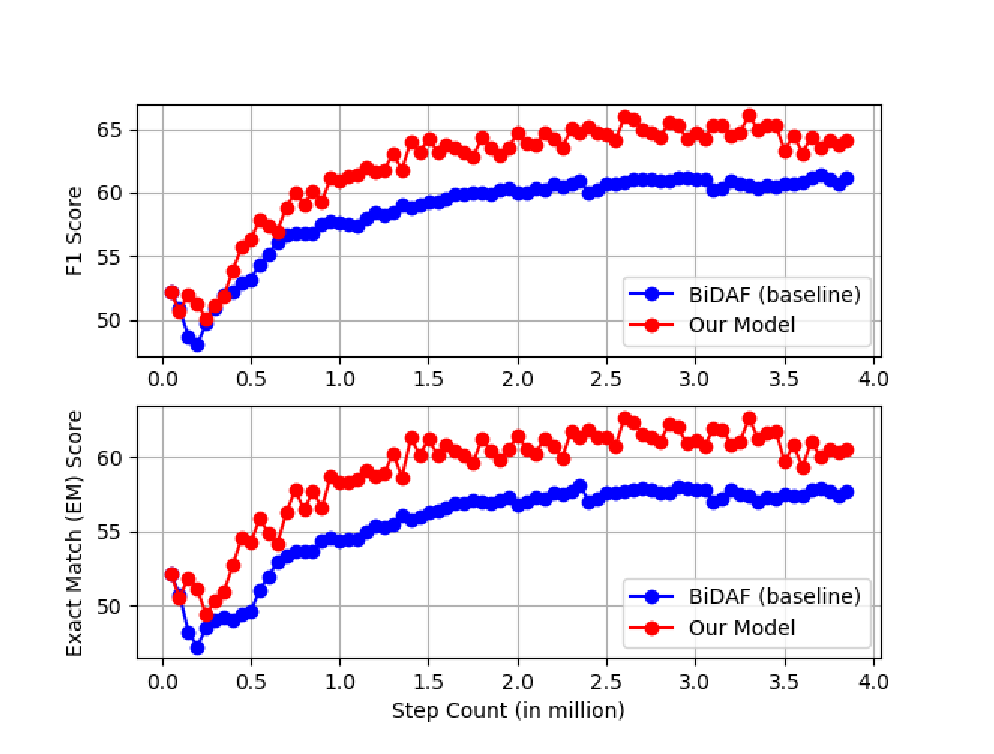
\includegraphics[width=12cm]{Figs4Paper/F1EM.eps}
  \caption{Comparison of F1 and EM scores}
  \label{fig:f1em}
\end{figure*}


\begin{table}[]
\caption{Comparing our model with the baseline}
\label{table:results}
\centering
\begin{tabular}{lll}
																									& EM    & F1    \\ \hline
BiDAF with character embedding (baseline)				  & 59.47 & 62.46 \\
Our Model																					& 62.64 & 66.10 \\ \hline

\end{tabular}
\end{table}

Table \ref{table:results} shows the comparison between our model and the baseline. As per the original BiDAF model, we include a character-level embedding layer using character-level convnets. This gives us a very strong baseline to compare with.


\subsection{Ablations}
\label{subsec:ablations}


\begin{table}[]
\caption{Results from Ablation Study}
\label{table:ablation}
\centering
\begin{tabular}{lll}
                                                                       & EM    & F1    \\ \hline
No Embedding Attention Layer                                           & 60.93 & 64.34 \\
No CNN layers inside the Embedding Encoder Layer                       & 59.64 & 63.10 \\
No character embedding in the Embedding Layer                          & 59.47 & 62.46 \\
Freezing both the character and word embeddings in the Embedding Layer & 62.19 & 65.39 \\ \hline

\end{tabular}
\end{table}


Table \ref{table:ablation} shows the performance of the model and its ablations on the SQuAD dev set. Having an Embedding Attention Layer helps model performance. This validates our hypothesis that adding attention layers early in the model stack should help performance. For ablating the effect of the CNN layers, we experiment by removing the CNN layers from the Embedding Encoder Layer. CNN layers prove to be critical with a drop of 3 points on both metrics. As noted by Seo at al \cite{seo2016bidirectional}, having character embeddings in the Embedding Layer contributes towards model performance whereby word-level embeddings represent the semantics of each word as a whole, while char-level embeddings better handle out-of-vocab (OOV) or rare words. Interestingly we also see that freezing the char-level and word-level embeddings gives us slightly lower performance. It seems the model gives slightly better results if we allow the backpropagation to happen all the way through the embedding layer, and the fine-tuned embeddings generalize quite well to unseen data in the dev set. 

\begin{table}[]
\caption{Effect of dropoput}
\label{table:dropoutresults}
\centering
\begin{tabular}{lll}
																	& EM    & F1    \\ \hline
No Dropout		   									& 60.41 & 63.46 \\
Dropout = 0.1    									& 62.06 & 65.39 \\ 
Dropout = 0.2 (chosen)		  			& 62.64 & 66.10 \\ 
Dropout = 0.3    									& 59.84 & 63.81 \\ 
Dropout = 0.4    									& 61.10 & 64.09 \\ \hline

\end{tabular}
\end{table}

Table \ref{table:ablation} shows the effect of dropout rates. With low dropout rates, the model was overfitting.  High drop-out rates help in preventing overfitting, but lead to lower EM/F1 scores. We settle on 0.2 as the dropout rate since it gave the best results.

% -----------------------------------------------
%\subsection{Implementation Details}
%\label{subsec:implementationdetails}

\begin{table}[]

    \caption{Preliminary Results}
    \label{table:results} 
    \centering
		
\begin{tabular}{|l|l|l|l|l|}
\hline
                                                                & \multicolumn{2}{l|}{\textbf{Dev Set}} & \multicolumn{2}{l|}{\textbf{Test Set}} \\ \hline
                                                                & EM                & F1                & EM                 & F1                \\ \hline
master                        				                          & 59.25             & 62.28             & 59.47              & 62.46             \\ \hline
baselinemodel\_selfsimilaritybeforeattention								 		& 58.83             & 62.05             & 57.47              & 60.87             \\ \hline
baselinemodel\_selfsimilarityafterattention								 			& 59.45             & 62.95             & 59.45              & 62.95             \\ \hline
conflict\_without\_for\_loops																 		& 55.67             & 59.19             & 55.67              & 59.19             \\ \hline
embedding\_with\_self\_similarity                               & 59.64             & 63.10             & 59.64              & 63.10             \\ \hline
embedding\_with\_self\_difference                               & 52.19             & 52.19             & 52.19              & 52.19             \\ \hline
conv\_rnn\_embed\_layer							                  	        & 60.93             & 64.34             & 60.93              & 64.34             \\ \hline
embedding\_with\_self\_similarity\_conv\_rnn (0.0)              & 62.19             & 65.26             & 60.41              & 63.46             \\ \hline
embedding\_with\_self\_similarity\_conv\_rnn (0.1)              & 62.19             & 65.26             & 62.06              & 65.39             \\ \hline
embedding\_with\_self\_similarity\_conv\_rnn (0.2)              & 62.19             & 65.26             & 62.19              & 65.26             \\ \hline
embedding\_with\_self\_similarity\_conv\_rnn (0.3)              & 62.19             & 65.26             & 59.84              & 63.18             \\ \hline
embedding\_with\_self\_similarity\_conv\_rnn (0.4)              & 62.19             & 65.26             & 61.10              & 64.09             \\ \hline
embedding\_with\_self\_similarity\_conv\_rnn (both unfrozen)    & 62.19             & 65.26             & 62.64              & 66.10             \\ \hline
\end{tabular}
		
\end{table}

